\section{Directory}
Tipicamente tutte le informazioni sui file vengono conservate nella struttura \textbf{directory}, che risiede sullo stesso dispositivo dei dati.
Al suo interno viene salvato, per ogni file, un identificatore e altri attributi:
\begin{sitemize}
    \item \textbf{Nome}
    \item \textbf{Tipo}
    \item \textbf{Indirizzo}
    \item \textbf{Lunghezza attuale}
    \item \textbf{Lunghezza massima}
    \item Data \textbf{ultimo accesso}
    \item Data \textbf{ultima modifica}
    \item \textbf{ID del proprietario}
    \item Informazioni di \textbf{protezione}
\end{sitemize}

\spacer
Sulla directory è possibile fare anche delle operazioni:
\begin{sitemize}
    \item \textbf{Ricerca}
    \item \textbf{Creazione} di un file
    \item \textbf{Eliminazione} di file
    \item \textbf{Elenco} di tutti i file
    \item \textbf{Ridenominazione} di un file
    \item \textbf{Attraversamento} del file system
\end{sitemize}

\spacer
La struttura dati della directory deve essere in grado di garantire buone prestazioni e deve permettere di raggruppare i file secondo specifiche caratteristiche.

\subsubsection*{Directory Monolivello}
La struttura più semplice è quella che pone tutti i file allo stesso livello.

Tuttavia questa struttura non supporta nessun raggruppamento logico e presenta problemi nel caso di due file con lo stesso nome.
\begin{figure}[H]
    \centering
    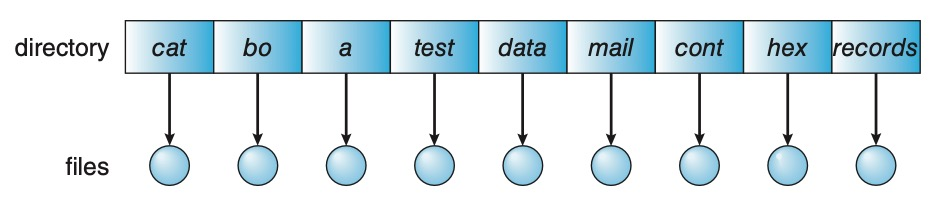
\includegraphics[width=0.5\linewidth]{assets/directory-monolivello.jpg}
\end{figure}

\subsubsection*{Directory a Due Livelli}
Ogni utente ha la sua directory ad un livello separata.

Questa struttura ha un possibile raggruppamento (per utente) ed non presenta problemi se due utenti hanno un file con lo stesso nome, tuttavia risulta essere ancora estremamente limitata.

\begin{figure}[H]
    \centering
    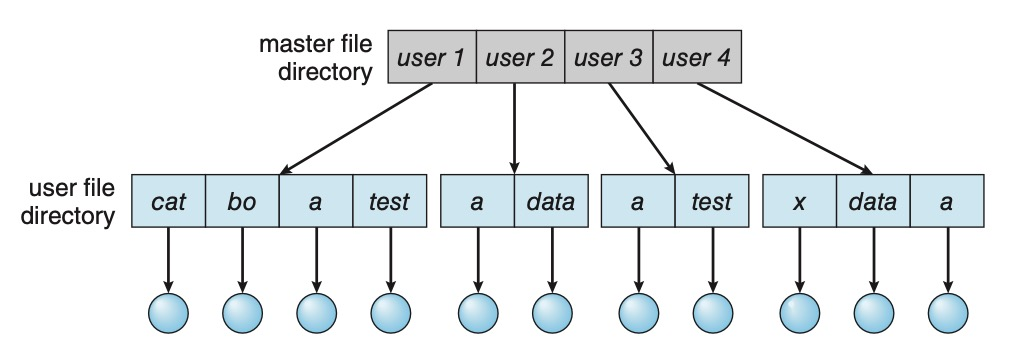
\includegraphics[width=0.5\linewidth]{assets/directory-2-livelli.jpg}
\end{figure}

\subsubsection*{Directory con struttura ad albero aciclico}
Una struttura ad albero è naturale per risolvere il problema della directory, infatti essa permette una ricerca rapida, un'ottima capacità di raggruppamento e permette file con lo stesso nome in directory diverse.

\spacer
Tutte le azioni (creazione di file, creazione di directory, cancellazione di directory) avvengono a partire da una directory.

\spacer
Un altro vantaggio della struttura ad albero è la possibilità di utilizzare più nomi diversi per indicare lo stesso file.
Questo può essere implementato solo come reference (soft link) oppure duplicando il file in memoria (hard link).

Questo porta a dei problemi per l'eliminazione del file, è necessario infatti eliminare anche tutte le reference. Viene quindi tenuto un counter delle reference ed il file non viene eliminato finché il counter non arriva a 0.

\begin{figure}[H]
    \centering
    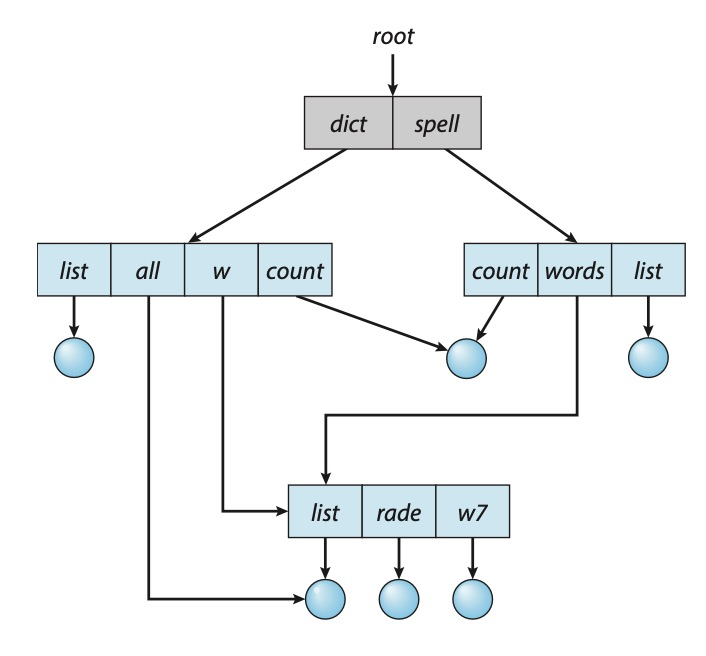
\includegraphics[width=0.42\linewidth]{assets/directory-albero-aciclico.jpg}
\end{figure}

\subsubsection*{Directory con struttura ad albero generale}
Se permettiamo anche la presenza di cicli nel grafo si ottengono dei problemi per l'attraversamento, vogliamo assicurarci che non ci siano file che vengono visitati due volte.

Per fare questo in fase di attraversamento è necessario marcare tutti i file visitati.

\spacer
Un'altra complicazione si trova nel fatto che un blocco può avere counter delle reference diverso da 0 pur non avendo nessun blocco che lo punta, per questo viene utilizzato un algoritmo di \textit{garbage collection} il quale attraversa l'albero e poi elimina tutti i file non contrassegnati come visitati.

\begin{figure}[H]
    \centering
    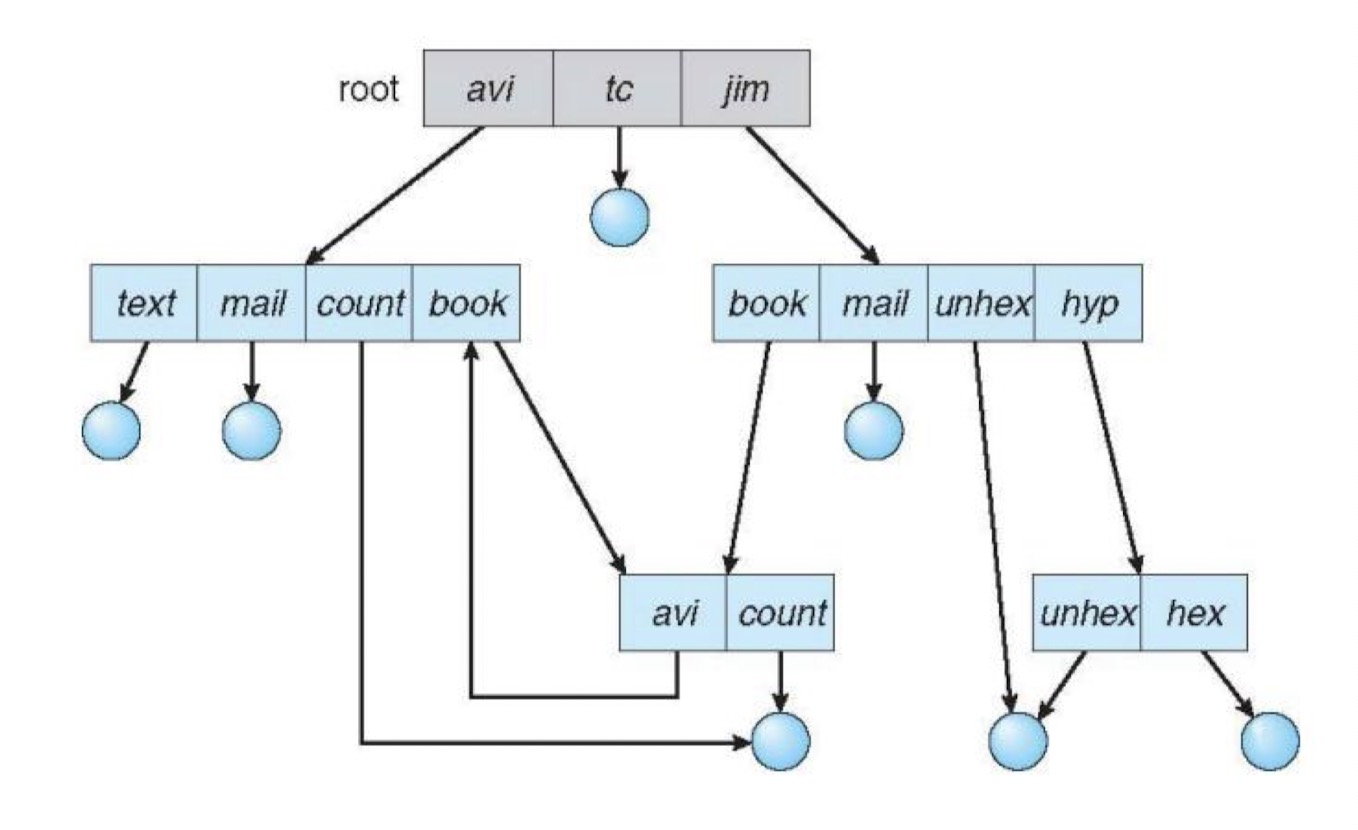
\includegraphics[width=0.42\linewidth]{assets/directory-grafo.jpg}
\end{figure}

\subsubsection*{Stabilire se un grafo è aciclico}
Per stabilire se un grafo è aciclico possiamo sfruttare il fatto che un grafo si dice aciclico se ha (almeno) un ordinamento topologico. Ovvero se è possibile assegnare ai nodi degli indici in modo che $$\forall \text{ ramo orientato } e = (u, v) \in G, index(u) < index(v)$$

Algoritmo per trovare un ordinamento topologico:
\begin{sitemize}
    \item Assegniamo (a caso) numeri crescenti ai vertici privi di rami entranti che non siano ancora numerati (se non ce ne sono, il grafo ha almeno un ciclo)
    \item Eliminiamo dal grafo i rami uscenti dai vertici a cui abbiamo assegnato un numero
    \item Ripetiamo finché ci sono vertici non numerati
\end{sitemize}

\begin{figure}[H]
    \centering
    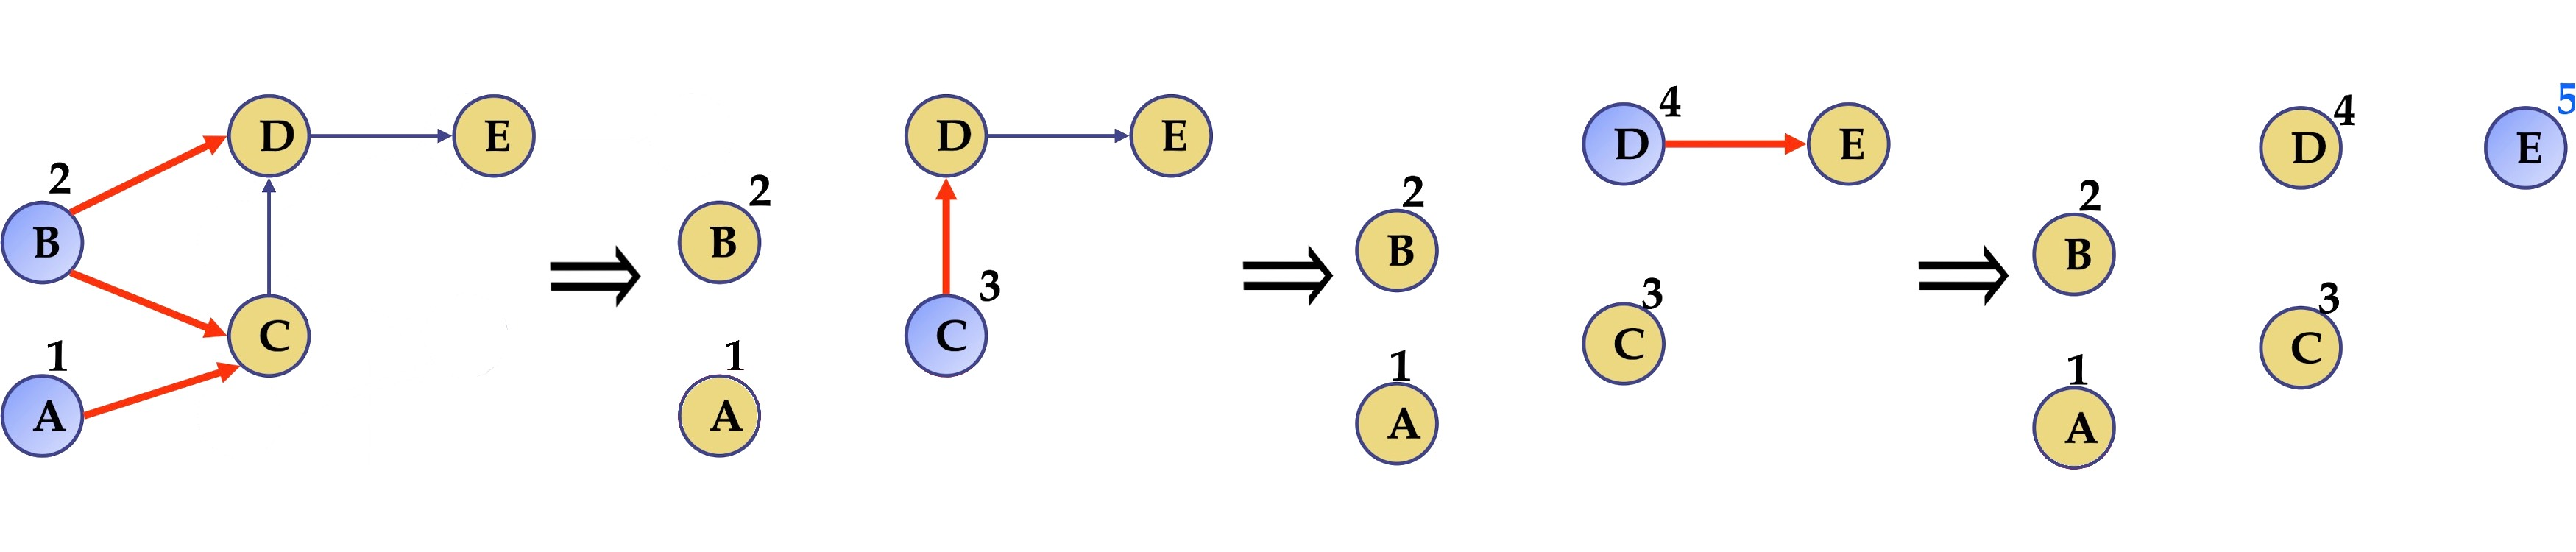
\includegraphics[width=0.75\linewidth]{assets/algoritmo-ordinamento-topologico.jpg}
\end{figure}

\subsubsection*{Implementazione}
La struttura dati può essere implementata tramite una lista o una lista concatenata, ma questa soluzioni ha importanti problemi sulle prestazioni.

Si preferisce utilizzare una tabella hash con chiave: nome del file, valore: puntatore all'identificatore del file. Essa porta a prestazioni migliori, anche se può avere necessità di rehash.

\subsection{Montaggio}
Per poter accedere ad un file system è necessario montarlo, ovvero attaccarne la struttura dati ad un punto di montaggio.

\spacer
La procedura richiede di fornire al sistema operativo il nome del dispositivo e il punto di montaggio, ovvero una directory a cui viene agganciato il file system.

Il punto di montaggio non deve essere una directory vuota, ma questo è preferibile in quanto i file in essa contenuti non saranno visibili fino all'operazione di unmount.

\spacer
I sistemi macOS e Windows rilevano tutti i dispositivi all'avvio e montano automaticamente tutti i loro file system.

Nei sistemi Unix è invece necessario montare i file system manualmente dopo l'avvio.

I sistemi Linux sono simili a quelli unix, ma forniscono anche un file di configurazione che permette di descrivere quali dispositivi montare in modo automatico.

\subsection{Esempi}
\subsubsection{Unix/Linux}
Viene costituito un grafo generale di directory, che ospita tutti i file e le directory.
A ciascun utente viene associata una directory come sottodirectory di \texttt{/usr}.

\spacer
Ciascun file viene identificato univocamente da un \textit{pathname}, questo significa che tutti i file e sottodirectory devono avere nomi distinti.

\spacer
Ogni utente che interagisce con il file system ha un proprio contesto, visualizzabile con \texttt{pwd} che può essere modificato grazie al comando \texttt{cd}.

\spacer
Esistono due tipi di link in linux, l'hard link che crea un nuovo elemento nella directory che punta allo stesso file fisico e il soft link che punta solamente ad un'altro elemento della directory.

Alla cancellazione dell'elemento gli hard link rimangono, mentre i soft link vengono tutti eliminati.

\spacer
Il comando \texttt{chmod} permette di modificare il livello di protezione assegnato al file.
È possibile utilizzare il comando per assegnare dei permessi sovrascrivendo quelli presenti o per modificare quelli già esistenti.

\begin{note}
    A partire da Fedora 33 è stato selezionato Btrfs come file system di default, esso fornisce dei servizi di pooling (risorse pronte per essere utilizzate), snapshots (una copia read only generata in O(1)) e checksum.
\end{note}
